\documentclass[17pt,a4paper,landscape]{extarticle}
\usepackage[margin=2.35cm,top=0.12cm,left=1.05cm]{geometry}
\usepackage{amsmath}
\usepackage{amssymb}
\usepackage{tasks}
\usepackage{tikz}
\usepackage{xcolor}
\usepackage[sfdefault,lf]{FiraSans}
\renewcommand{\familydefault}{\sfdefault}
\setlength{\parindent}{0pt}
\pagestyle{empty}
\settasks{label=\textbf{\arabic*.}, label-width=2.2em, item-indent=2.95em, column-sep=2.1cm, after-item-skip=4.7em}
\renewcommand{\arraystretch}{1.15}
\everymath{\displaystyle}

\begin{document}
\sffamily
\boldmath

\boldmath

{\LARGE \textbf{Naming angles --- Foundation}}
\begin{tasks}(3)
\task {Name the marked angle.\\[0.4em]
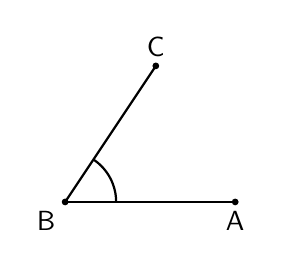
\begin{tikzpicture}[scale=0.72,baseline=(current bounding box.center)]
  \coordinate (B) at (0,0); \coordinate (A) at (3.0,0); \coordinate (C) at (1.6,2.4);
  \draw[thick] (B)--(A); \draw[thick] (B)--(C);
  \draw[thick] (0.9,0) arc[start angle=0,end angle=56,radius=0.9];
  \fill (A) circle (1.7pt) node[below] {A}; \fill (B) circle (1.7pt) node[below left] {B}; \fill (C) circle (1.7pt) node[above] {C};
\end{tikzpicture}}
\task {Name the marked angle.\\[0.4em]
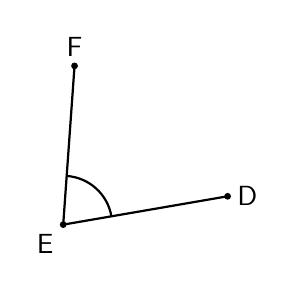
\begin{tikzpicture}[scale=0.72,baseline=(current bounding box.center)]
  \coordinate (E) at (0,0); \coordinate (D) at (2.9,0.5); \coordinate (F) at (0.2,2.8);
  \draw[thick] (E)--(D); \draw[thick] (E)--(F);
  \draw[thick] (0.85,0.15) arc[start angle=10,end angle=86,radius=0.86];
  \fill (D) circle (1.7pt) node[right] {D}; \fill (E) circle (1.7pt) node[below left] {E}; \fill (F) circle (1.7pt) node[above] {F};
\end{tikzpicture}}
\task {Name the marked angle.\\[0.4em]
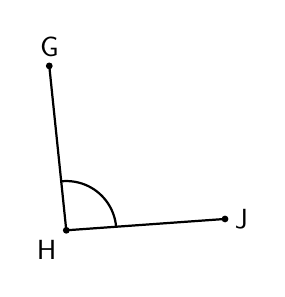
\begin{tikzpicture}[scale=0.72,baseline=(current bounding box.center)]
  \coordinate (H) at (0,0); \coordinate (G) at (-0.3,2.9); \coordinate (J) at (2.8,0.2);
  \draw[thick] (H)--(G); \draw[thick] (H)--(J);
  \draw[thick] (0.88,0.05) arc[start angle=4,end angle=96,radius=0.88];
  \fill (G) circle (1.7pt) node[above] {G}; \fill (H) circle (1.7pt) node[below left] {H}; \fill (J) circle (1.7pt) node[right] {J};
\end{tikzpicture}}
\task {Circle the letter that is the vertex in \mbox{$\angle PQR$}.\\[0.3em]A. \mbox{$P$} \quad B. \mbox{$Q$} \quad C. \mbox{$R$}}
\task {Circle the letter that is the vertex in \mbox{$\angle MNO$}.\\[0.3em]A. \mbox{$M$} \quad B. \mbox{$N$} \quad C. \mbox{$O$}}
\task {Which name matches the angle shown?\\[0.4em]
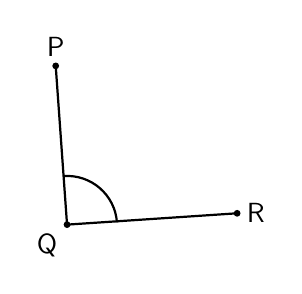
\begin{tikzpicture}[scale=0.72,baseline=(current bounding box.center)]
  \coordinate (Q) at (0,0); \coordinate (P) at (-0.2,2.8); \coordinate (R) at (3.0,0.2);
  \draw[thick] (Q)--(P); \draw[thick] (Q)--(R);
  \draw[thick] (0.88,0.04) arc[start angle=4,end angle=94,radius=0.88];
  \fill (P) circle (1.7pt) node[above] {P}; \fill (Q) circle (1.7pt) node[below left] {Q}; \fill (R) circle (1.7pt) node[right] {R};
\end{tikzpicture}\\[0.2em]A. \mbox{$\angle PQR$} \quad B. \mbox{$\angle PRQ$} \quad C. \mbox{$\angle QPR$}}
\task {Which name matches the angle shown?\\[0.4em]
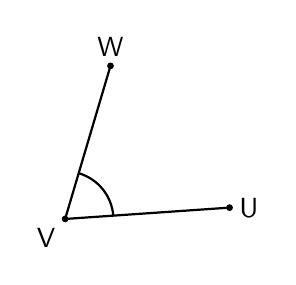
\begin{tikzpicture}[scale=0.72,baseline=(current bounding box.center)]
  \coordinate (V) at (0,0); \coordinate (U) at (2.9,0.2); \coordinate (W) at (0.8,2.7);
  \draw[thick] (V)--(U); \draw[thick] (V)--(W);
  \draw[thick] (0.85,0.05) arc[start angle=4,end angle=74,radius=0.85];
  \fill (U) circle (1.7pt) node[right] {U}; \fill (V) circle (1.7pt) node[below left] {V}; \fill (W) circle (1.7pt) node[above] {W};
\end{tikzpicture}\\[0.2em]A. \mbox{$\angle UVW$} \quad B. \mbox{$\angle VWU$} \quad C. \mbox{$\angle WUV$}}
\task {Fill in the missing letter so the vertex is \mbox{$B$}: \mbox{$\angle A\underline{\hspace{0.8cm}}C$}}
\task {Fill in the missing letter so the vertex is \mbox{$S$}: \mbox{$\angle R\underline{\hspace{0.8cm}}T$}}
\task {Write another correct name for the same angle: \mbox{$\angle ABC = \underline{\hspace{3cm}}$}}
\task {Write another correct name for the same angle: \mbox{$\angle DEF = \underline{\hspace{3cm}}$}}
\task {Explain this rule in a few words: where does the vertex go when naming an angle?}
\end{tasks}

\end{document}
